%   ===================================================
%	Plotting the LR and short-run equilibria after
%    a change in demand
%
%   A: Original LR equilibrium 
%   B: SR equilibrium after change in demand
%   C: New LR equilibrium once entry/exit resumes
%
%   Author: Patrick Blanchenay
%   ===================================================

\documentclass{standalone}
% =============================================
\usepackage{tikz}               % to draw things
\usepackage{pgfplots}           % to draw plots & curves
\pgfplotsset{compat=1.8}
\usetikzlibrary{calc,intersections}  % to find and define intersections of curves, equilibria...
% ---------------------------------------------------------------------
% Coordinate extraction % https://tex.stackexchange.com/questions/420498/extract-convert-store-and-reuse-x-y-coordinate-components/426245#426245
% #1: node name
% #2: output macro name: x coordinate
% #3: output macro name: y coordinate
\newcommand{\Getxycoords}[3]{%
	\pgfplotsextra{%
		% using `\pgfplotspointgetcoordinates' stores the (axis)
		% coordinates in `data point' which then can be called by
		% `\pgfkeysvalueof' or `\pgfkeysgetvalue'
		\pgfplotspointgetcoordinates{(#1)}%
		% `\global' (a TeX macro and not a TikZ/PGFPlots one) allows to
		% store the values globally
		\global\pgfkeysgetvalue{/data point/x}{#2}%
		\global\pgfkeysgetvalue{/data point/y}{#3}%
	}%
}
\tikzset{ % to make dots on the graph
dot/.style = {circle, fill, minimum size=#1,
           inner sep=0pt, outer sep=0pt},
dot/.default = 6pt % size of the circle diameter 
}
% =============================================
\begin{document}

% ========= Things to change ======================
  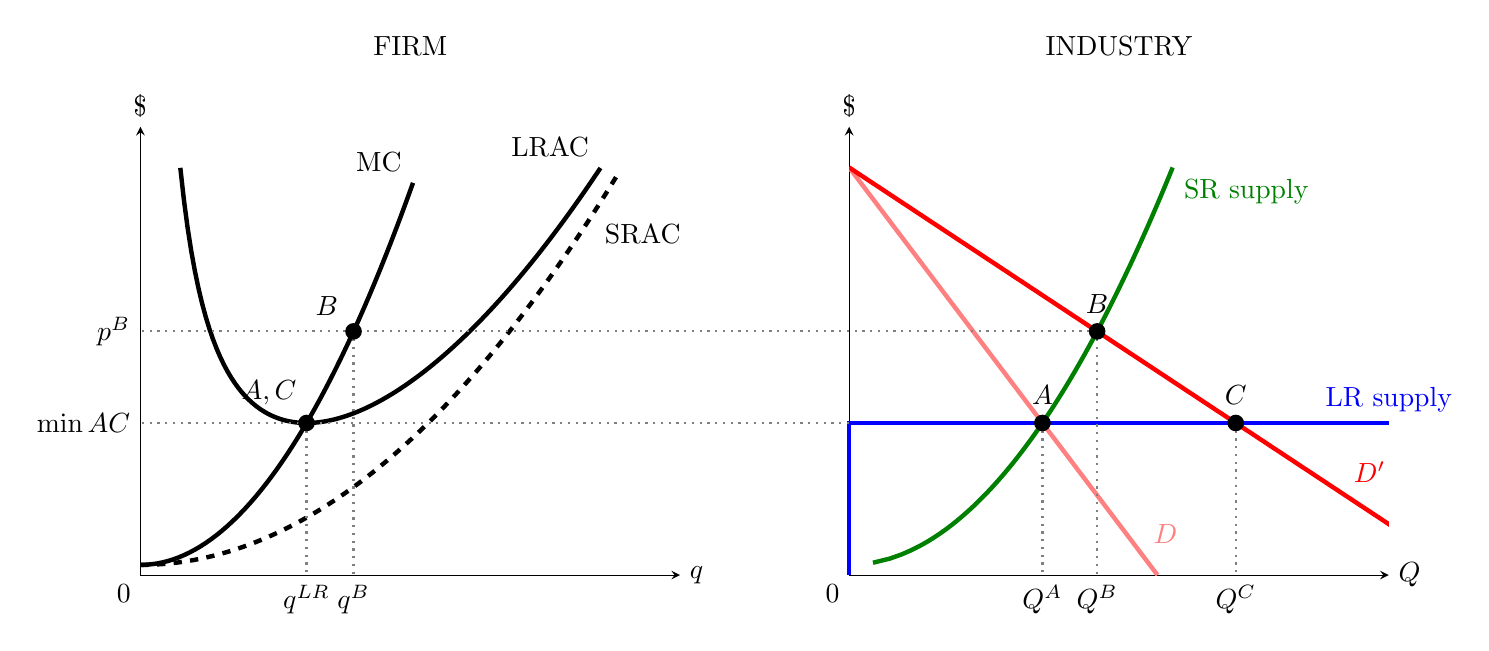
\begin{tikzpicture}[
  	declare function={
  		demandfunction(\p)      =   800-20*\p;      % Original demand
  		newdemandfunction(\p)   =   1600-40*\p;  % New demand
  	}] % 

% Cost functions (bassed on cost function q^3 +q+ 20)
	\def\lrac{q^2+1+20/q}  % Long-run Average Cost of a single firm
	\def\srac{q^2+1}       % Short-run Average Cost of a single firm (Fixed cost is sunk)
	\def\lrmc{3*q^2+1}     % Marginal Cost
	\def\supplysinglefirm{sqrt((p-1)/3)} % From inverting MC(q)=p
% Graph settings
	\def\pmax{40}          % Maximum price to display on the vertical axis
	\def\qmaxsinglefirm{7} % Maximum quantity supply for a single firm
	\def\qmaxindustry{1400} % Maximum quantity supply for the industry
% ======= GRAPH HAPPENS HERE =========== 
% SINGLE FIRM   
    \begin{axis}[   scale=1,
    	title style={at={(0.5,1)},anchor=north,yshift=30},
     	title = {FIRM},
       	axis lines=middle, xlabel style={right }, ylabel style={above },
       	xlabel=$q$, ylabel=\textdollar, 
       	xmin=0.0,xmax=\qmaxsinglefirm, % quantities
       	ymin=0.0,ymax=\pmax, % price
       	restrict y to domain=0:\pmax,
       	xtick=\empty, 
       	ytick=\empty,
  		enlarge y limits={upper=0.15},
% 		enlarge x limits={upper=0.5},
 		clip mode=individual,
       	]
  
       % LRMC	
       \addplot[name path global=lrmc,samples=100,, ultra thick,domain=0:\qmaxsinglefirm,variable=q] (q,\lrmc) node[above left,pos=1] {MC}; 
      % LRAC	
      \addplot[name path global=lracsingle,samples=150,, ultra thick,domain=0:\qmaxsinglefirm,variable=q] (q,\lrac) node[above left,pos=1] {LRAC}; 
       % SRAC	
       \addplot[name path global=sracsingle,dashed,samples=150, ultra thick,domain=0:\qmaxsinglefirm,variable=q] (q,\srac) node[below right,pos=0.9] {SRAC}; 
    
     	% Axes origin
     	\node [below left] (origin) at (axis cs:0,0) {$0$};	
		\coordinate (verticalaxis) at (axis cs:0,\pmax); 
		\coordinate (horizontalaxis) at (axis cs:\qmaxsinglefirm,0); 

     	% Finds the single firm min AC point and EQUILIBRIUM
    	 \path [name intersections={of=lracsingle and lrmc,by=LROriginalEquilSingle}]; % LR equillibrium for single firms   
     	\coordinate (minacsinglestart) at (LROriginalEquilSingle -| verticalaxis) {}; % compute min AC on vertical axis
     	
     	\Getxycoords{LROriginalEquilSingle}{\LRsingleq}{\LRsingleprice} % Useful to find number of firms in original LR equil

   \end{axis}
   
   \pgfmathsetmacro{\nbfirmsinitial}{demandfunction(\LRsingleprice)/\LRsingleq} % Calculates nb firms initially present in LR equil
   
   % INDUSTRY
   \begin{axis}[   scale=1,xshift=9cm, % xshift used to put another graph next to it
       		title style={at={(0.5,1)},anchor=north,yshift=30},
        	title = {INDUSTRY},
          	axis lines=middle, xlabel style={right }, ylabel style={above },
          	xlabel=$Q$, ylabel=\textdollar, 
          	xmin=0.0,xmax=\qmaxindustry, % quantities
          	ymin=0.0,ymax=\pmax, % price
          	restrict y to domain=0:\pmax,
          	xtick=\empty,
          	ytick=\empty,
     		enlarge y limits={upper=0.15},
   % 		enlarge x limits={upper=0.5},
    		clip mode=individual,
          	]

	        % ORIGINAL DEMAND
	        \addplot[name path global=demand,samples=10,red!50, ultra thick,domain=\pmax:0,variable=p] 
	          	(demandfunction(p),p)  node[above right ,pos=0.95] {$D$}; 
	        % NEW DEMAND
          	\addplot[name path global=newdemand,samples=10,red, ultra thick,domain=\pmax:0,variable=p] 
          	 	(newdemandfunction(p),p) node[above right,pos=0.8] {$D'$};    
 
        	% Axes origin & axes
        	\node [below left] (origin) at (axis cs:0,0) {$0$};	
        	\coordinate (verticalaxisindustry) at (axis cs:0,\pmax); 
        	\coordinate (horizontalaxisindustry) at (axis cs:\qmaxindustry,0); 
           	
        	% LR SUPPLY 
        	\coordinate (minacindustrystart) at (LROriginalEquilSingle -| verticalaxisindustry) ; % compute min AC and vertical axis
			\coordinate (minacindustryend) at (minacindustrystart -| horizontalaxisindustry) ; % compute min AC and all the way to the right
        	\draw[name path global=lraggsupply,very thick, blue] (axis cs:0,0)--(minacindustrystart) -- (minacindustryend) node[above ,pos=1] {LR supply};

         	% LR EQUILIBRIA
   			\path [name intersections={of=lraggsupply and demand,by=LROriginalEquil}]; %  LR equil before shift in demand      	
     		\path [name intersections={of=lraggsupply and newdemand,by=LRNewEquil}]; % LR equil after shift in demand
     	
       		% SR SUPPLY and EQUILIBRIUM
	      	\addplot[name path global=sraggsupply,samples=100,green!50!black, ultra thick,domain=0:\pmax,variable=p] 
	      		( \nbfirmsinitial  *   \supplysinglefirm,p) node[below right,pos=1] {SR supply};  	       
   	    	\path [name intersections={of=sraggsupply and newdemand,by=SRNewEquil}]; % SR equil after shift in demand
     	

   
      \end{axis}
% Project points on the axes
% INDUSTRY QUANTITIES
\draw[thick,gray,dotted]  (LROriginalEquil) -- (LROriginalEquil |- horizontalaxisindustry) node[below,black] {$Q^A$}  ;
\draw[thick,gray,dotted]  (SRNewEquil) -- (SRNewEquil |- horizontalaxisindustry) node[below,black] {$Q^B$}  ;
\draw[thick,gray,dotted]  (LRNewEquil) -- (LRNewEquil |- horizontalaxisindustry) node[below,black] {$Q^C$}  ;
% PRICES
\draw[thick,gray,dotted,name path global=SRpriceline]  (SRNewEquil) -- (SRNewEquil -| verticalaxis) node[left,black] {$p^B$}  ;
\draw[thick,gray,dotted] (minacsinglestart -| verticalaxisindustry) --  (minacsinglestart) node[left,black] {$\min AC$}   ;
\path [name intersections={of=lrmc and SRpriceline,by=srsupplysingle}]; % SR supply after shift in demand  
% SINGLE FIRM QUANTITIES
\draw[thick,gray,dotted]  (LROriginalEquilSingle) -- (LROriginalEquilSingle |- horizontalaxis) node[below,black] {$q^{LR}$}  ;
\draw[thick,gray,dotted]  (srsupplysingle) -- (srsupplysingle |- horizontalaxis) node[below,black] {$q^B$}  ; % SR equil single
% Place dots and label equilibria
\node[dot,label=135:{$B$},fill]  at (srsupplysingle) {};
\node[dot,label=93:{$A,C$},fill]  at (LROriginalEquilSingle) {};
\node[dot,label=90:$A$,fill]  at (LROriginalEquil) {};
\node[dot,label=90:$B$,fill]  at (SRNewEquil) {};
\node[dot,label=90:$C$,fill]  at (LRNewEquil) {};

\end{tikzpicture}

% =============================================	
\end{document}